\documentclass[notes,11pt, aspectratio=169, xcolor=table]{beamer}

\usepackage{pgfpages}
% These slides also contain speaker notes. You can print just the slides,
% just the notes, or both, depending on the setting below. Comment out the want
% you want.
\setbeameroption{hide notes} % Only slide
%\setbeameroption{show only notes} % Only notes
%\setbeameroption{show notes on second screen=right} % Both

\usepackage{helvet}
\usepackage[default]{lato}
\usepackage{array}
\usepackage{minted}

\newtheorem{proposition}{Proposition}

\usepackage{tikz}
\usetikzlibrary{shapes.geometric}
\usepackage{pgfplots}
\usepackage{graphicx}
\usepackage{verbatim}
\setbeamertemplate{note page}{\pagecolor{yellow!5}\insertnote}
\usetikzlibrary{positioning}
\usetikzlibrary{snakes}
\usetikzlibrary{calc}
\usetikzlibrary{arrows}
\usetikzlibrary{decorations.markings}
\usetikzlibrary{shapes.misc}
\usetikzlibrary{matrix,shapes,arrows,fit,tikzmark}
\usepackage{amsmath}
\usepackage{mathpazo}
\usepackage{hyperref}
\usepackage{lipsum}
\usepackage{multimedia}
\usepackage{graphicx}
\usepackage{multirow}
\usepackage{graphicx}
\usepackage{dcolumn}
\usepackage{bbm}
\usepackage[style=authoryear,sorting=nyt,uniquename=false]{biblatex}

\addbibresource{references.bib} 

\newcolumntype{d}[0]{D{.}{.}{5}}

\def\@@mybluebox[#1][#2]#3{
    \sbox\mytempbox{#3}%
    \mytemplen\ht\mytempbox
    \advance\mytemplen #1\relax
    \ht\mytempbox\mytemplen
    \mytemplen\dp\mytempbox
    \advance\mytemplen #2\relax
    \dp\mytempbox\mytemplen
    \colorbox{myblue}{\hspace{1em}\usebox{\mytempbox}\hspace{1em}}}


\usepackage{changepage}
\usepackage{appendixnumberbeamer}
\newcommand{\beginbackup}{
   \newcounter{framenumbervorappendix}
   \setcounter{framenumbervorappendix}{\value{framenumber}}
   \setbeamertemplate{footline}
   {
     \leavevmode%
     \hline
     box{%
       \begin{beamercolorbox}[wd=\paperwidth,ht=2.25ex,dp=1ex,right]{footlinecolor}%
%         \insertframenumber  \hspace*{2ex} 
       \end{beamercolorbox}}%
     \vskip0pt%
   }
 }
\newcommand{\backupend}{
   \addtocounter{framenumbervorappendix}{-\value{framenumber}}
   \addtocounter{framenumber}{\value{framenumbervorappendix}} 
}


\usepackage{graphicx}
\usepackage[space]{grffile}
\usepackage{booktabs}

% These are my colors -- there are many like them, but these ones are mine.
\definecolor{blue}{RGB}{0,114,178}
\definecolor{red}{RGB}{213,94,0}
\definecolor{yellow}{RGB}{240,228,66}
\definecolor{green}{RGB}{0,158,115}

\hypersetup{
  colorlinks=false,
  linkbordercolor = {white},
  linkcolor = {blue}
}


%% I use a beige off white for my background
\definecolor{MyBackground}{RGB}{255,253,218}

%% Uncomment this if you want to change the background color to something else
%\setbeamercolor{background canvas}{bg=MyBackground}

%% Change the bg color to adjust your transition slide background color!
\newenvironment{transitionframe}{
  \setbeamercolor{background canvas}{bg=yellow}
  \begin{frame}}{
    \end{frame}
}

\setbeamercolor{frametitle}{fg=blue}
\setbeamercolor{title}{fg=blue}
\setbeamertemplate{footline}[frame number]
\setbeamertemplate{navigation symbols}{} 
\setbeamertemplate{itemize items}{-}
\setbeamercolor{itemize item}{fg=blue}
\setbeamercolor{itemize subitem}{fg=blue}
\setbeamercolor{enumerate item}{fg=blue}
\setbeamercolor{enumerate subitem}{fg=blue}
\setbeamercolor{button}{bg=MyBackground,fg=blue,}



% If you like road maps, rather than having clutter at the top, have a roadmap show up at the end of each section 
% (and after your introduction)
% Uncomment this is if you want the roadmap!
% \AtBeginSection[]
% {
%    \begin{frame}
%        \frametitle{Roadmap of Talk}
%        \tableofcontents[currentsection]
%    \end{frame}
% }
\setbeamercolor{section in toc}{fg=blue}
\setbeamercolor{subsection in toc}{fg=red}
\setbeamersize{text margin left=1em,text margin right=1em} 

\newenvironment{wideitemize}{\itemize\addtolength{\itemsep}{10pt}}{\enditemize}

\usepackage{environ}
\NewEnviron{videoframe}[1]{
  \begin{frame}
    \vspace{-8pt}
    \begin{columns}[onlytextwidth, T] % align columns
      \begin{column}{.58\textwidth}
        \begin{minipage}[t][\textheight][t]
          {\dimexpr\textwidth}
          \vspace{8pt}
          \hspace{4pt} {\Large \sc \textcolor{blue}{#1}}
          \vspace{8pt}
          
          \BODY
        \end{minipage}
      \end{column}%
      \hfill%
      \begin{column}{.42\textwidth}
        \colorbox{green!20}{\begin{minipage}[t][1.2\textheight][t]
            {\dimexpr\textwidth}
            Face goes here
          \end{minipage}}
      \end{column}%
    \end{columns}
  \end{frame}
}

\title[]{International Trade: Lecture 2}
\subtitle[]{Trade with Data}
\author[Góes]
{Carlos Góes\inst{1}}
\date{Fall 2025}
\institute[GWU]{\inst{1} George Washington University }



\begin{document}

%%% TIKZ STUFF
\tikzset{   
        every picture/.style={remember picture,baseline},
        every node/.style={anchor=base,align=center,outer sep=1.5pt},
        every path/.style={thick},
        }
\newcommand\marktopleft[1]{%
    \tikz[overlay,remember picture] 
        \node (marker-#1-a) at (-.3em,.3em) {};%
}
\newcommand\markbottomright[2]{%
    \tikz[overlay,remember picture] 
        \node (marker-#1-b) at (0em,0em) {};%
}
\tikzstyle{every picture}+=[remember picture] 
\tikzstyle{mybox} =[draw=black, very thick, rectangle, inner sep=10pt, inner ysep=20pt]
\tikzstyle{fancytitle} =[draw=black,fill=red, text=white]
%%%% END TIKZ STUFF



%----------------------------------------------------------------------%
%-------------------       TITLE PAGE       ---------------------------%
%----------------------------------------------------------------------%





%----------------------------------------------------------------------%






%----------------------------------------------------------------------%
%----------------------------------------------------------------------%

%----------------------------------------------------------------------%
\frame{\titlepage}
\addtocounter{framenumber}{-1}
%----------------------------------------------------------------------%



%----------------------------------------------------------------------%
%----------------------------------------------------------------------%

\section{Introduction to Python}

\subsection{Why Python?}

    \begin{frame}{Why Python?}
    \framesubtitle{Python for data science}
        
        \begin{itemize}
          \item Python is a \textbf{general‑purpose programming language} that is growing in popularity both in data science and other fields.
          \item Python prioritizes code readability for humans—and it is very easy for beginners.
          \item It follows principles such as (see the \textit{Zen of Python}):
             \begin{itemize}
                \item Explicit is better than implicit;
                \item Simple is better than complex;
                \item Readability counts.
            \end{itemize}
        \end{itemize}

    \end{frame}
    
    \begin{frame}[fragile=singleslide]{Why Python?}
    \framesubtitle{Easy to understand}

    \begin{block}{Java}
        \begin{minted}{java}
            class myprog
            {
                public static void main(String args[])
                {
                    System.out.println("Oi!");
                }
            }
                    \end{minted}
    \end{block}
    
    \begin{alertblock}{Python}
        \begin{minted}{python}
            print("Oi!")
        \end{minted}
    \end{alertblock}

    \end{frame}

    \begin{frame}{Introduction to Spyder}
    \framesubtitle{How to use Spyder?}
        
        \begin{figure}
            \begin{center}
                \colorbox{white}{
                    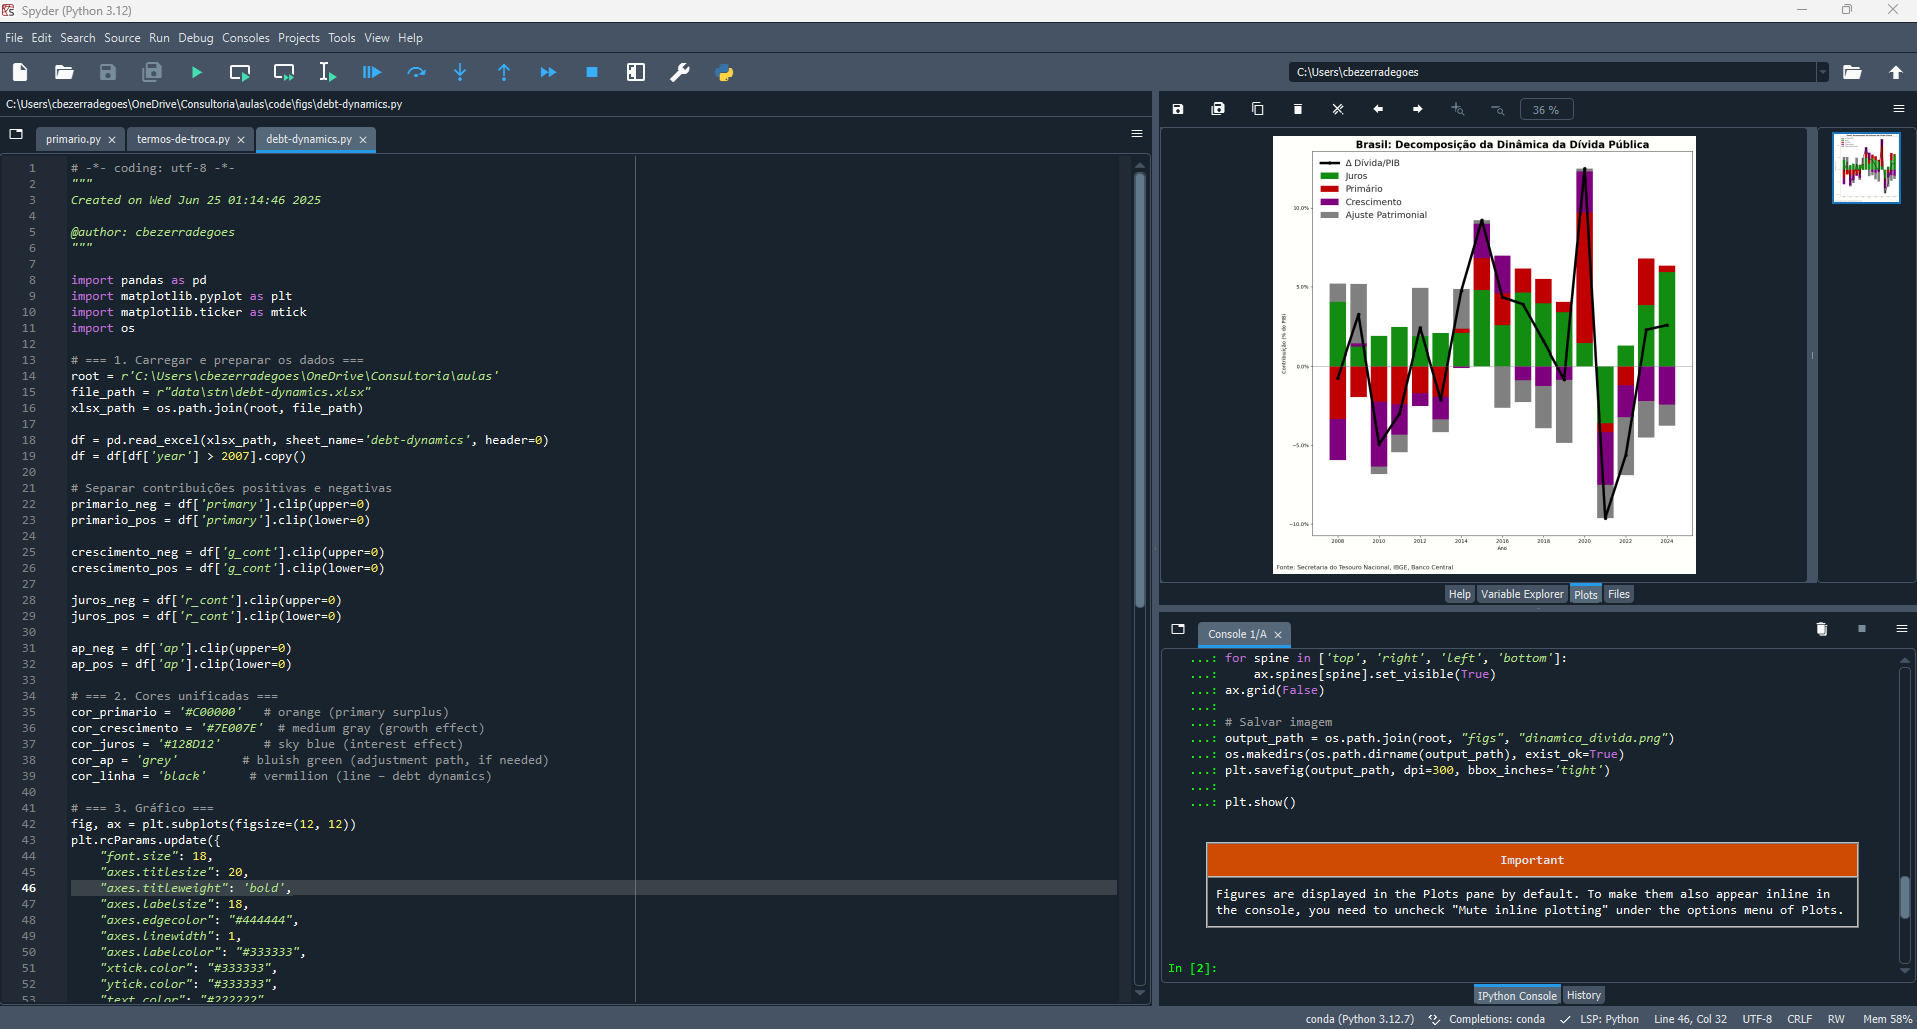
\includegraphics[scale=0.2]{figs/spyder.PNG} 
                }
            \end{center}
            \caption[Diagrama de Conway]{\textbf{Spyder.} Componentes do IDE. \label{fig:spyder}}
        \end{figure}  

    
   

    \end{frame}

\subsection{Integers, floats, strings and booleans}  

    \begin{frame}[fragile=singleslide]{Integers, floats, strings and booleans}
    \framesubtitle{Integers}

        \begin{itemize}
            \item \mintinline{python}{Integers} are \textit{whole numbers} (no decimals or fractions).
            \begin{equation}
                \mathbb{Z} \quad \equiv \quad \{ \hdots, -3, -2, -1, 0, 1, 2, 3, \hdots \}
            \end{equation}
             
            \item Example in Python:
        \end{itemize}

        \begin{minted}{python}
        
            var = 20
            print(type(var))
        \end{minted}    
   

    \end{frame}
    
    \begin{frame}[fragile=singleslide]{Integers, floats, strings and booleans}
    \framesubtitle{Floats}

        \begin{itemize}
            \item \mintinline{python}{Floats} are arithmetic representations of all \textit{real} numbers.
            \begin{eqnarray}
                \mathbb{R} &\quad& \equiv \quad \{ \hdots, -\pi, -2.5, -\sqrt{2}, -\frac{1}{2}, 0, \frac{1}{2}, \sqrt{2}, 2.5, \pi, \hdots \} \\ \nonumber
                \mathbb{R} &\quad& \equiv \quad \{ \hdots, -3.14159265, -2.5, -1.41421356, \\ \nonumber
                &\qquad& -0.5, 0, 0.5, 1.41421356, 2.5, 3.14159265, \hdots \}
            \end{eqnarray}
            \item Example in Python:
        \end{itemize}

        \begin{minted}{python}
        
            var = 3.14159265
            print(type(var))
        \end{minted}    
   

    \end{frame}    

    \begin{frame}[fragile=singleslide]{Integers, floats, strings and booleans}
    \framesubtitle{Strings}

        \begin{itemize}
            \item \mintinline{python}{Strings} are text representations.
            \item Example in Python:
        \end{itemize}

        \begin{minted}{python}
        
            var = "Esse é um string"
            print(type(var))
        \end{minted}    
   

    \end{frame}    

    \begin{frame}[fragile=singleslide]{Integers, floats, strings and booleans}
    \framesubtitle{Booleans}

        \begin{itemize}
            \item \mintinline{python}{Booleans} are logical representations (true or false).
            \item Example in Python:
        \end{itemize}

        \begin{minted}{python}
            var1 = True
            print(type(var1))
            var2 = (2+2 == 5)
            print(type(var2))
        \end{minted}    
   
    \end{frame}    

    \begin{frame}[fragile=singleslide]{Integers, floats, strings and booleans}
    \framesubtitle{Variable types and theoretical categorizations}

        \begin{itemize}
            \item Discrete quantitative variables: \mintinline{python}{integers}.
            \item Continuous quantitative variables: \mintinline{python}{floats}.
            \item Categorical qualitative variables: \mintinline{python}{booleans} or \mintinline{python}{strings}.
            \item Ordinal qualitative variables: \mintinline{python}{strings} or \mintinline{python}{integers}.
        \end{itemize}
    \end{frame}    
    

    \begin{frame}[fragile=singleslide]{Integers, floats, strings and booleans}
    \framesubtitle{Numeric operations}

        \begin{itemize}
            \item Addition:
                \begin{minted}{python}
                    x + y
                \end{minted}    
            \item Subtraction:
                \begin{minted}{python}
                    x - y
                \end{minted}    
            \item Division:
                \begin{minted}{python}
                    x / y
                \end{minted}    
            \item Multiplication:
                \begin{minted}{python}
                    x * y
                \end{minted}    
            \item Exponentiation:
                \begin{minted}{python}
                    x ** y
                \end{minted}    
            \item Modulo (remainder):
                \begin{minted}{python}
                    x % y
                    3 % 2 is 1
                \end{minted}    
        \end{itemize}

    \end{frame}      

    \begin{frame}[fragile=singleslide]{Integers, floats, strings and booleans}
    \framesubtitle{String operations}

        \begin{itemize}
            \item Addition:
                \begin{minted}{python}
                str1 = "Carlos"
                str2 = "Góes"
                print(str1 + " " + str2)
                \end{minted}    
            \item Multiplication:
                \begin{minted}{python}
                str1 = "a"
                print(str1 * 10)
                \end{minted}    
        \end{itemize}

    \end{frame}          

    \begin{frame}[fragile=singleslide]{Integers, floats, strings and booleans}
    \framesubtitle{Logical operations}

        \begin{itemize}
            \item Equality:
                \begin{minted}{python}
                2 + 2 is 4
                2 + 2 == 4
                str = "a"
                str is "a"
                str == "a"
                \end{minted}    
            \item Inequality:
                \begin{minted}{python}
                2 + 2 is not 4
                2 + 2 != 4
                str = "a"
                str is not "a"
                str != "a"
                \end{minted}    
            \item Greater than or less than:
                \begin{minted}{python}
                10 > 100
                10 < 100
                \end{minted}    
        \end{itemize}

    \end{frame}              
    
        \begin{frame}[fragile=singleslide]{Integers, floats, strings and booleans}
    \framesubtitle{Logical operations}

        \begin{itemize}
            \item In logical operations, \mintinline{python}{True} has the numeric value 1 and \mintinline{python}{False} has the numeric value 0; you can use this to perform arithmetic.
            \item Sum (how many are true?):
                \begin{minted}{python}
                a = 1 + 1 is 2
                b = 2 * 2 is 4
                c = 2 * 2 is 5
                d = a + b + c
                print(d)
                \end{minted}    
            \item Product (are all true?):
                \begin{minted}{python}
                a = 1 + 1 is 2
                b = 2 * 2 is 4
                c = 2 * 2 is 5
                d = a * b * c
                print(d)
                \end{minted}    
        \end{itemize}

    \end{frame}              
    
\subsection{Lists and dictionaries}  

    \begin{frame}[fragile=singleslide]{Lists and dictionaries}
    \framesubtitle{Lists}
    
         \begin{itemize}
            \item \mintinline{python}{Lists} are collections of variables defined with \mintinline{python}{[square brackets]} and elements separated by commas:

                \begin{minted}{python}
                lista1 = [2, 20.5, "Oi!", 10 < 100] 
                print(lista1)
                \end{minted}    

            \item \mintinline{python}{Lists} are indexed from $0$ to the last element; access an element with the syntax \mintinline{python}{list_name[index]}.
            
            \item For example, \mintinline{python}{print(lista1[0])} returns \mintinline{python}{2}.
            
            \item Meanwhile, \mintinline{python}{print(lista1[3])} returns \mintinline{python}{True}.

        \end{itemize}       

    \end{frame}

    \begin{frame}[fragile=singleslide]{Lists and dictionaries}
    \framesubtitle{Lists}
    
         \begin{itemize}
            \item You can change a list element by assigning a value to a specific index:

                \begin{minted}{python}
                lista1[0]= 20 
                print(lista1)
                \end{minted}    

            \item Add an element to the list:

                \begin{minted}{python}
                lista1.append(79.2) 
                print(lista1)
                \end{minted}    

            \item Use multiplication to repeat the contents of a list:

                \begin{minted}{python}
                lista2 = lista1 * 2 
                print(lista2)
                \end{minted}    

            \item Or use addition to concatenate two lists:

                \begin{minted}{python}
                lista3 = [1,2]
                lista4 = [5,6]
                lista5 = lista3 + lista4
                print(lista5)
                \end{minted}    

        \end{itemize}       

    \end{frame}

    \begin{frame}[fragile=singleslide]{Lists and dictionaries}
    \framesubtitle{Dictionaries}
        
         \begin{itemize}
            \item \mintinline{python}{Dictionaries} are, as the name suggests, collections of key–value pairs; unlike lists, dictionaries are indexed by keys (usually words):

                \begin{minted}{python}
                pessoa1 = {
                        'nome': 'Milton Friedman',
                        'nascimento': '31/07/1912'
                        }
                print(pessoa1)
                print(pessoa1['nome'])
                \end{minted}    

            \item Add an element to the dictionary:

                \begin{minted}{python}
                pessoa1.update({'nacionalidade': 'EUA'})
                print(pessoa1)
                \end{minted}    

        \end{itemize}             

    
   

    \end{frame}

    \section{Introduction to \mintinline{python}{pandas}}

        \subsection{Comandos básicos}

        \begin{frame}[fragile=singleslide]{Introduction to \mintinline{python}{pandas}}
        \framesubtitle{Importing the \mintinline{python}{pandas}}
            
             \begin{itemize}
    
                \item The \mintinline{python}{pandas} package must be installed first!
                
                \item After that we can simply import it:
    
                    \begin{minted}[fontsize=\footnotesize]{python}
                     import pandas as pd
                    \end{minted}
                    
                \item \mintinline{python}{pandas} has two basic structures: \mintinline{python}{Series} and \mintinline{python}{DataFrames}; the latter are collections of the former.
                    
            \end{itemize}             
    
        \end{frame}
        
        \begin{frame}[fragile=singleslide]{Introduction to \mintinline{python}{pandas}}
        \framesubtitle{\mintinline{python}{Series}}
            
             \begin{itemize}
    
                \item \mintinline{python}{Series} are built from other objects:
    
                    \begin{minted}[fontsize=\footnotesize]{python}
                     x = np.linspace(1,10, 5)
                     rotulo = ["a","b","c","d","e"]
                     serie1 = pd.Series(x, name="Série1", index=rotulo)
                     print(serie1)
                    \end{minted}
                    
                \item Like \mintinline{python}{lists}, you can access an element of a \mintinline{python}{Series} using its index:
                
                \begin{minted}[fontsize=\footnotesize]{python}
                    print(serie1["a"])
                    print(serie1["d"])
                \end{minted}
                
                    
            \end{itemize}             
    
        \end{frame}    

        \begin{frame}[fragile=singleslide]{Introduction to \mintinline{python}{pandas}}
        \framesubtitle{\mintinline{python}{Series}}
            
             \begin{itemize}
    
                \item If you build your \mintinline{python}{Series} from \mintinline{python}{dictionaries}, they already come with indexes:
    
                    \begin{minted}[fontsize=\footnotesize]{python}
                    matricula  = {
                        'Carlos Goes': '06/99209',
                        "Nicolas Powidayko": '10/22290',
                        "Alexander Rabbat": '08/21346',
                        "Dani Alaino": '07/20345',
                        "Lya Nikate": '09/23567',
                        "Niz Borroz": '11/22035',
                        "Tom Rundal": "98/20145"
                    }
                    
                    serie2 = pd.Series(matricula)
                    print(serie2)

                    \end{minted}
                
                    
            \end{itemize}             
    
        \end{frame}    

        \begin{frame}[fragile=singleslide]{Introduction to \mintinline{python}{pandas}}
        \framesubtitle{\mintinline{python}{DataFrames}}
            
             \begin{itemize}
    
                \item \mintinline{python}{DataFrames} are groups of \mintinline{python}{Series}:
    
                    \begin{minted}[fontsize=\footnotesize]{python}
                     x = np.linspace(1,10, 5)
                     y = np.linspace(1,20, 5)
                     rotulo = ["a","b","c","d","e"]
                     serie1 = pd.Series(x, name="Série1", index=rotulo)
                     serie2 = pd.Series(y, name="Série2", index=rotulo)
                     
                     df = pd.DataFrame(data=[serie1, serie2])
                    \end{minted}
                    
                \item You can extract both columns and rows:
                
                \begin{minted}[fontsize=\footnotesize]{python}
                    print(df["a"])
                    print(df.loc["Série1"])
                \end{minted}

                \item And transpose (flip) the data:
                
                \begin{minted}[fontsize=\footnotesize]{python}
                    print(df.T)
                \end{minted}
                    
            \end{itemize}             

        \end{frame}    

        \begin{frame}[fragile=singleslide]{Introduction to \mintinline{python}{pandas}}
        \framesubtitle{\mintinline{python}{DataFrames}}
            
             \begin{itemize}
    
                \item You can also grab a specific element inside a column: \mintinline{python}{print(df["a"]["Series1"])}

                \item Or call the row first and then the column: \mintinline{python}{print(df.loc["Series1"]["a"])}
        
            \end{itemize}             

        \end{frame}    

        \begin{frame}[fragile=singleslide]{Introduction to \mintinline{python}{pandas}}
        \framesubtitle{\mintinline{python}{DataFrames}}
            
             \begin{itemize}
    
                \item Let’s create a \mintinline{python}{DataFrame} with several attributes:

                    \begin{minted}[fontsize=\tiny]{python}
                    matricula = pd.Series(matricula)
                    
                    curso = pd.Series({
                            'Carlos Goes': 'Economia',
                            "Nicolas Powidayko": 'Economia',
                            "Alexander Rabbat": 'Ciência da Computação',
                            "Dani Alaino": 'Ciência da Computação',
                            "Lya Nikate": 'Ciência da Computação',
                            "Niz Borroz": 'Estatística',
                            "Tom Rundal": "Ciência da Computação"
                            })

                    ira = pd.Series({
                            'Carlos Goes': 5.0,
                            "Nicolas Powidayko": 4.8,
                            "Alexander Rabbat": 3.8,
                            "Dani Alaino": 4.4,
                            "Lya Nikate": 4.3,
                            "Niz Borroz": 4.0,
                            "Tom Rundal": 4.0
                            })

                    lista = [matricula, curso, ira]
                    df = pd.DataFrame(lista, index=['matricula', 'curso', 'ira']).T
                    \end{minted}
        
            \end{itemize}             

        \end{frame}    

        \begin{frame}[fragile=singleslide]{Introduction to \mintinline{python}{pandas}}
        \framesubtitle{\mintinline{python}{DataFrames}}
            
             \begin{itemize}
    
                \item How to extract the attributes of Carlos Goes? \mintinline{python}{df.loc["Carlos Goes"]}

                \item How to extract all registration numbers? \mintinline{python}{df["matricula"]}
                
                \item How to extract the data for all Computer Science students?
                
                \begin{itemize}
                    \item \textit{Boolean masking}!
                    \item Try: \mintinline{python}{print(df["curso"] == "Ciência da Computação")}
                    \item And now like this: \mintinline{python}{print(df[ df["curso"] == "Ciência da Computação" ])}
                    \item What happened?
                \end{itemize}
        
            \end{itemize}             

        \end{frame}    
            
        \subsection{How to import a file?}

        \begin{frame}[fragile=singleslide]{Introdução ao Pandas}
        \framesubtitle{How to import a file?}
            
             \begin{itemize}
    
                \item Answer: it depends on the type of file you are importing.
                
                \item File types:
                
                    \begin{itemize}
                        \item \textbf{Spreadsheet}: .xls, .xlsx, etc.
                        \item \textbf{Text}: .txt, .csv, .tsv, etc.
                        \item \textbf{JSON} or \textbf{SQL}: .json, .sql
                        \item Others...
                    \end{itemize}
                    
            \end{itemize}             
    
        \end{frame}        

        \begin{frame}[fragile=singleslide]{Introdução ao Pandas}
        \framesubtitle{How to import a file?}
            
             \begin{itemize}
    
                \item Here we will work with a text file, which is very common in data analysis.

                \item Visit this website and see how the data are organized: \url{https://raw.githubusercontent.com/omercadopopular/cgoes/master/piketty/fdatabasetax.csv}

                \item Now let’s import it:
                
                \begin{minted}[fontsize=\footnotesize]{python}
                url = "https://raw.githubusercontent.com/      \
                       omercadopopular/cgoes/master/piketty/   \
                       fdatabasetax.csv"
                
                piketty = pd.read_csv(url)
                print(piketty.head())
                \end{minted}
                
                    
            \end{itemize}             
    
        \end{frame}        
        \subsection{How to extract descriptive statistics?}

        \begin{frame}[fragile=singleslide]{Introdução ao Pandas}
        \framesubtitle{How to extract descriptive statistics?}
            
             \begin{itemize}
    
                \item Mean, median and quartiles
                
                    \begin{minted}[fontsize=\footnotesize]{python}
                     estd = pd.DataFrame([piketty.mean(),
                                         piketty.min(),
                                         piketty.quantile(0.25),
                                         piketty.median(),
                                         piketty.quantile(0.75)
                                         piketty.max()],
                                         
                                         index=['média', 'min',
                                                'Q1', 'mediana,
                                                'Q3', 'max'])
                     
                     print(estd)
                    \end{minted}
                
                \item Or:
                
                
                    \begin{minted}[fontsize=\footnotesize]{python}
                     piketty.describe()
                    \end{minted}
                
                    
            \end{itemize}             

    \end{frame}        

        \subsection{How to limit the sample?}
        
        \begin{frame}[fragile=singleslide]{Introdução ao Pandas}
        \framesubtitle{How to limit the sample?}
            
             \begin{itemize}
    
                \item Country
                    \begin{minted}[fontsize=\footnotesize]{python}
                     australia = piketty[
                        piketty['country'] == "Australia"
                     ]
                    \end{minted}

                \item Year
                    \begin{minted}[fontsize=\footnotesize]{python}
                     y2000 = piketty[ piketty['year'] == 2000 ]
                    \end{minted}
                    
            \end{itemize}             

    \end{frame}        

        \subsection{How to limit the sample?}
        
        \begin{frame}[fragile=singleslide]{Introdução ao Pandas}
        \framesubtitle{How to limit the sample?}
            
             \begin{itemize}
    
                \item Grouping (aggregating) by categories
                    \begin{minted}[fontsize=\footnotesize]{python}
                    mean = (piketty
                            .groupby('country')
                            .mean())
                    \end{minted}
                    \begin{minted}[fontsize=\footnotesize]{python}
                    sum = (piketty
                            .groupby('country')
                            .sum())
                    \end{minted}
                    
            \end{itemize}             

    \end{frame}           
    
    
\end{document}
